\documentclass[a4paper,11pt]{article}

\usepackage[english]{babel}
\usepackage[utf8x]{inputenc}
\usepackage{amsmath}
\usepackage{graphicx}
\usepackage[margin=0.5in]{geometry}
\usepackage{caption}
\usepackage{subcaption}


\begin{document}

{\Huge TSC1 Notes}

\hfill\rule{150mm}{.1pt}

\hfill{\small \today}

\section{Example 1}
Consider a block sliding down a frictionless ramp.  The system is assumed to be conservative, so
$$
\frac{mv^2}{2} = mgh = mg d\sin\theta = mg vt\sin^2 \theta
$$
where $v$ is the velocity of the block, $t$ is the time the block has been in motion, $m$ is the mass of the block, $g$ is the local acceleration due to gravity, $h$ is the height of the block before it is released, and $d$ is the distance the block has traveled.  The velocity is then  
$$
v(t) = 2gt\sin^2 \theta\;\;.
$$
If the angle of the ramp is varied with time as
$$
\theta(t) = \sin(t)\;\;,
$$
then it is expected that $\theta(t)\rightarrow v(t)$, i.e.\ the changing angle drives the changing magnitude of the velocity.

The angle driving signal and the velocity response signal are seen in Figure \ref{fig:thetaandv}.
\begin{figure}[ht]
\begin{tabular}{ll}
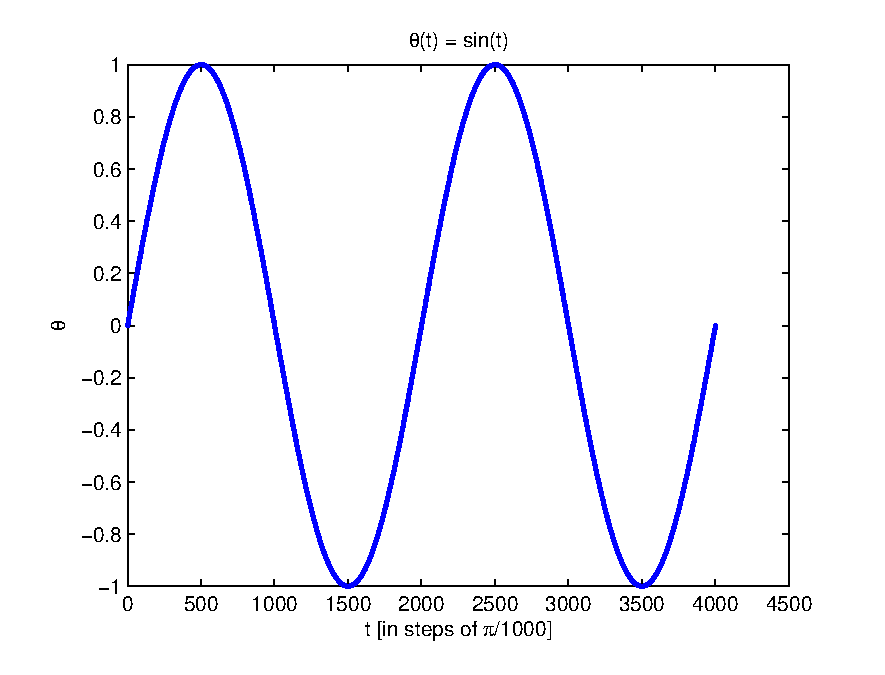
\includegraphics[scale=0.65]{theta.eps} & 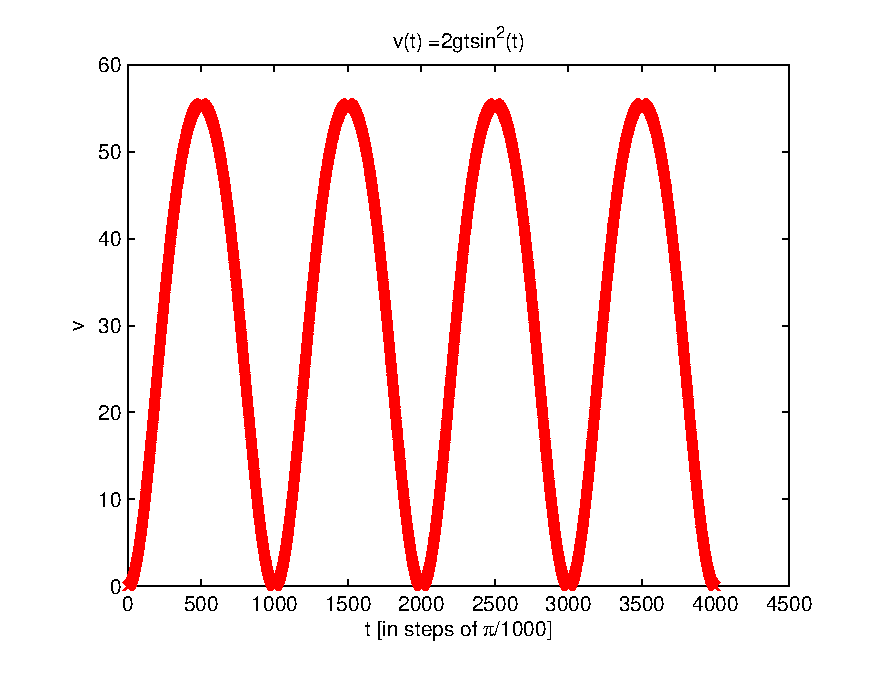
\includegraphics[scale=0.65]{v.eps}\\
\end{tabular}
\caption{}
\label{fig:thetaandv}
\end{figure}

The change in $\theta$ is expected to affect $v$, so a first step is to find the distribution of changes in $\theta$; i.e.\
$$
\delta\theta(t) \equiv \frac{d\theta}{dt} \approx \frac{\Delta\theta}{\Delta t} = \theta(t)-\theta(t-1)\;\;.
$$
A histogram of $\{\delta\theta(t)\;|\;t\ge 0\}$ is seen in Figure \ref{fig:dthetahist}.
\begin{figure}[ht]
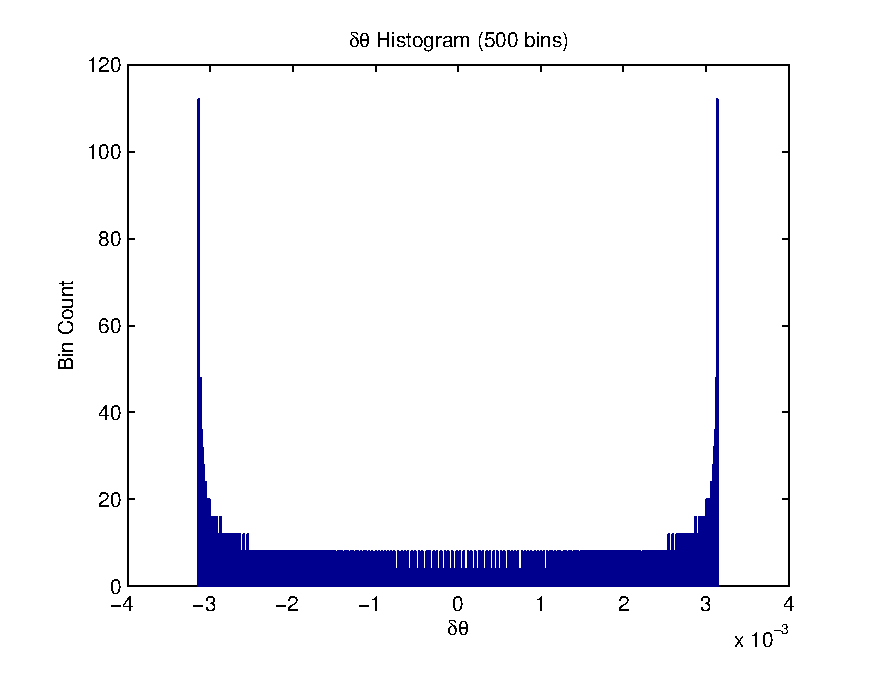
\includegraphics[scale=0.65]{dthetahist.eps}
\caption{}
\label{fig:dthetahist}
\end{figure}
A given bin can be picked (e.g.\ bin 125 in Figure \ref{fig:dthetahist}), and the values of $v$ that occur immediately following the binned $\delta\theta$ can be plotted to give an idea of how the response signal reacts to the given change in the driving signal.  Let $B_i = \{t_k\}$ be the set of times $t$ corresponding to the $i$th bin of $\delta\theta$ which contains all the $\{\delta\theta(t_k)\}$ that belong to that bin.  The plot of the correspondingly binned response signal would be a plot of $\{v(t+1)\;|\; t\in B_i\}$.  Figure \ref{fig:vbin125} is such a plot for $B_{125}$.
\begin{figure}[ht]
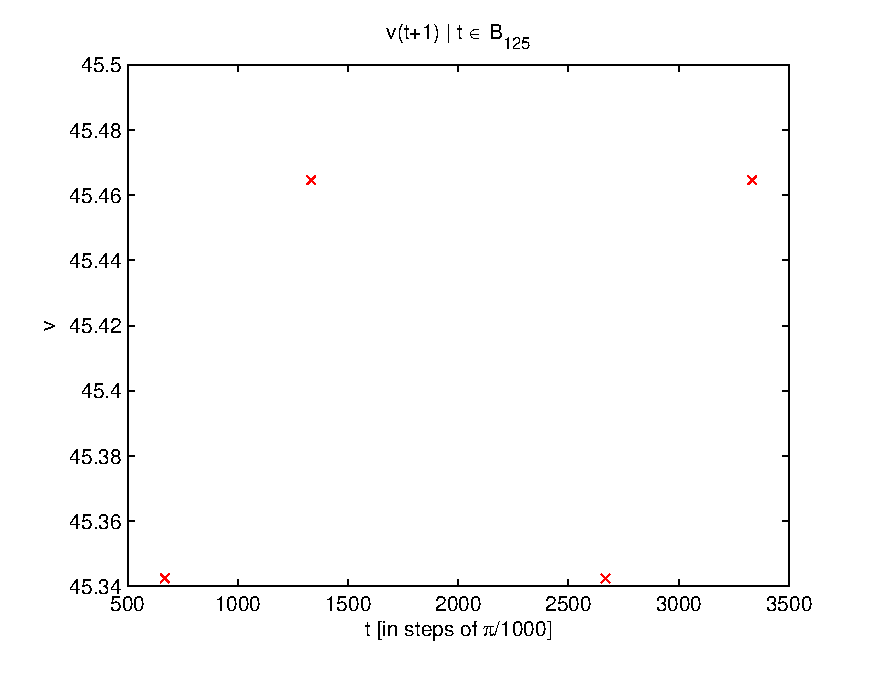
\includegraphics[scale=0.65]{vbin125.eps}
\caption{}
\label{fig:vbin125}
\end{figure}

Conceptually, the response signal is expected to have only a few different values in response to a given change in the driver.  However, it might be expected that the actual value of the response might also depend on the previous value of the response signal.  For example, a $0.25\pi$ change in $\theta$ would lead to a different value of $v(t)$ depending on $v(t-1)$.  Two ways to approach this problem are to define a change in $v$ (i.e.\ $\delta v$) and then investigate $\{\delta v(t+1)\;|\; t\in B_i\}$ or to bin $v$ and then investigate $\delta\theta$-binned response values $v$ within a given $v$-binned set.  Both methods are explored below.

\subsection{$\delta\theta$ leads to $\delta v(t)$}
The set $\{\delta\theta(t_k)\;\forall t_k\in B_i\}$ can be compared with $\{\delta v(t_k+1)\}$ to understand how similar changes in $\theta$ are followed by changes in $v$.  Figure \ref{fig:dthetadv} shows such a plot for $i=125$.
\begin{figure}[ht]
\begin{tabular}{ll}
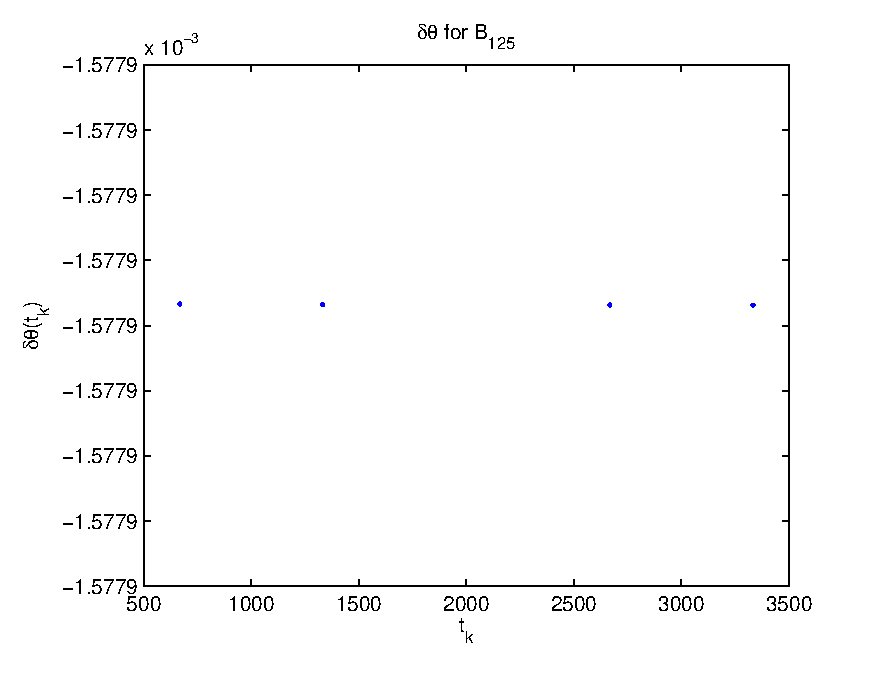
\includegraphics[scale=0.65]{dthetabin125.eps} & 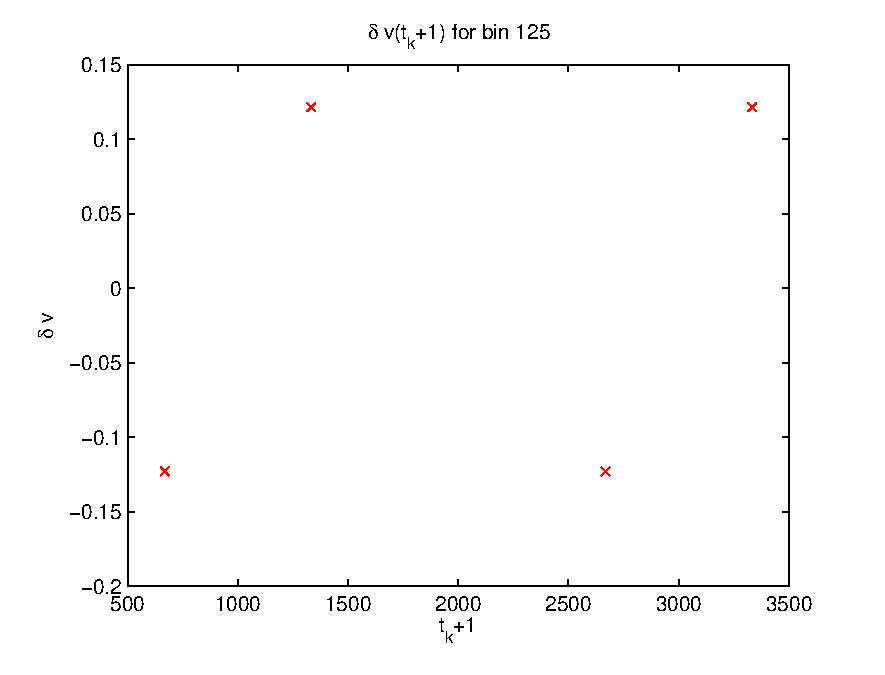
\includegraphics[scale=0.65]{dvbin125.eps}\\
\end{tabular}
\caption{}
\label{fig:dthetadv}
\end{figure}
The figures show that for $B_{125}$ two separate values of $\delta v(t_k+1)$ seem to follow $\delta\theta(t_k)$.  From above,
$$
\delta\theta(t_k) = \theta(t_k)-\theta(t_k-1) = \sin(t_k) - \sin(t_k-1)
$$
and
\begin{eqnarray*}
\delta v(t_k+1) &=& v(t_k+1)-v(t_k)\\
&=& 2g\left(\left(t_k+1\right)\sin^2 \left(\theta(t_k+1)\right) - \left(t_k\right)\sin^2 \left(\theta(t_k)\right) \right)\\
&=& 2g\left(\left(t_k+1\right)\sin^2 \left(\sin(t_k+1)\right) - \left(t_k\right)\sin^2 \left(\sin(t_k)\right) \right)
\end{eqnarray*}

Consider $t_k = n\pi$ where $n=0,1,2,\ldots$.  
$$
\delta\theta(n\pi) = \sin(n\pi) - \sin(n\pi-1) = -\left(-\sin(1)\right) = \sin(1)
$$
\begin{eqnarray*}
\delta v(n\pi+1) &=& 2g\left(\left(n\pi+1\right)\sin^2 \left(\sin(n\pi+1)\right) - \left(n\pi\right)\sin^2 \left(\sin(n\pi)\right) \right)\\
&=& 2g\left(n\pi+1\right)\sin^2 \left(\sin(1)\right)\\
\end{eqnarray*}
Thus, the histogram bin that contains $\delta\theta = \sin(1)$ would include the points recorded at the set of time steps $\{t_k = n\pi\}$, i.e.\ $\{\delta\theta(n\pi)\}\subseteq H_i$.  The set of $\delta v$ that immediately follow the points in $H_i$, i.e.\ $\{\delta v(n\pi+1)\}$, will contain $n$ points, as does $H_i$ if $\{\delta\theta(n\pi)\}= H_i$.  However, the value of the points in $\{\delta\theta(n\pi)\}$ is all the same (i.e.\ $\sin(1)$), whereas the values of the points in $\{\delta v(n\pi+1)\}$ increase monotonically in $n$.  

Consider $t_k = n\pi/2$ where $n=1,3,5,\ldots$.  
\begin{eqnarray*}
\delta\theta\left(\frac{n\pi}{2}\right) &=& \sin\left(\frac{n\pi}{2}\right) - \sin(\frac{n\pi}{2}-1)\\
&=& 1-\cos(1) \;\;\;\;\mathrm{(n = 1,5,9,...)}\\
&=& -1-\left(-\cos(1)\right) = \cos(1)-1 \;\;\;\;\mathrm{(n = 3,7,11,...)}
\end{eqnarray*}
\begin{eqnarray*}
\delta v(\frac{n\pi}{2}+1) &=& 2g\left(\left(\frac{n\pi}{2}+1\right)\sin^2 \left(\sin(\frac{n\pi}{2}+1)\right) - \left(\frac{n\pi}{2}\right)\sin^2 \left(\sin(\frac{n\pi}{2})\right) \right)\\
&=& 2g\left(\left(\frac{n\pi}{2}+1\right)\sin^2 \left(1-\cos(1)\right) - \left(\frac{n\pi}{2}\right)\sin^2 \left(-1\right) \right)\;\;\;\;\mathrm{(n = 1,5,9,...)}\\
&=& 2g\left(\left(\frac{n\pi}{2}+1\right)\sin^2 \left(\cos(1)-1\right) - \left(\frac{n\pi}{2}\right)\sin^2 \left(1\right) \right)\;\;\;\;\mathrm{(n = 3,7,11,...)}\\
\end{eqnarray*}
Again, the value of the points in $\{\delta\theta(n\pi/2)\}$ are all the same (depending on the sign), whereas the values of the points in $\{\delta v(n\pi/2+1)\}$ are not constant.

Thus, the change in the velocity, $v$, {\em caused} by a given change in the ramp angle, $\theta$ may depend on the cycle location of the system (i.e.\ $n$).  This observation, even at just the one special time step considered here, implies that it may be difficult to determine causality by comparing changes in the ramp angle to changes in the velocity.  Determining causality requires isolating the effect of a change in the driver (in this case $\theta$).  If the response (in this case $v$) can have many different responses based on other system parameters (in this case cycle location), then isolating the effect of the driver in the response would require controlling for all the other system parameters, which are expected to be unknown.

The lack of knowledge about potential system parameters is a major problem in time series causality.  Often it is not just the values of system parameters that are unknown but rather their existence.  How many parameters are there in the system that produced the response signal?  What could they possible be?  Can they be controlled for? Etc.  These complications suggest that a more straightforward approach may just be to control for the values of the response system itself.  

\subsection{Subsetting $\delta\theta$ and $v$: Local Impulse Response Inference (??)}

Consider the $t_k=n\pi$ example from the previous subsection.  The set $\{\delta\theta(n\pi)\}$ contains $n$ points.  Consider
\begin{eqnarray*}
v(n\pi-1) &=& 2g\left(n\pi-1\right)\sin^2 \left(\theta(n\pi-1)\right)\\
&=& 2g\left(n\pi-1\right)\sin^2 \left(\sin(n\pi-1)\right)\\
&=& 2g\left(n\pi-1\right)\sin^2 \left(-\sin(1)\right)\\
&=& 2g\left(n\pi-1\right)\left(-1\right)^2\sin^2 \left(\sin(1)\right)\\
&=& 2g\left(n\pi-1\right)\sin^2 \left(\sin(1)\right)
\end{eqnarray*}
The set $\{v(n\pi-1)\}$ will have $n$ points.  Performing a histogram on this set will effectively be subsetting by $n$ because the values in the set $\{v(n\pi-1)\}$ are only a function of $n$.  This is a key idea: a histogram of the response signal values immediately preceding a given change in the driver is considered equivalent to subsetting by (i.e.\ ``controlling for'') the unknown system parameters.

For this example, consider an $n$-binned histogram of $\{v(n\pi-1)\}$, which implies a single value is in each bin.  Consider the bin $n=1$ which contains the value $v(\pi-1)=2g\left(\pi-1\right)\sin^2 \left(\sin(1)\right)$.  For this bin, the driver changes by $\delta\theta(\pi)=\sin(1)$ (as it would for all the bins).  The response signal immediately following the change in the driver is 
\begin{eqnarray*}
v(t_k+1) = v(\pi+1) &=& 2g\left(\pi+1\right)\sin^2 \left(\theta(\pi+1)\right)\\
&=& 2g\left(\pi+1\right)\sin^2 \left(\sin(\pi+1)\right)\\
&=& 2g\left(\pi+1\right)\sin^2 \left(\sin(1)\right)\;\;.
\end{eqnarray*}
The set $\{v(\pi+1)\}$ contains a single point, and thus the effect of a change in the driving signal $\theta$ has been isolated by controlling for the values of the response $v$ that precede the change.  The algorithm is straightforward to describe as 1.\ create $\delta\theta$, 2.\ create histogram $\mathbf{H}_\theta$ of $\delta\theta$, and 3. for each bin of $\mathbf{H}_\theta$ create histogram of preceding $v$.  

The question is now how to define causality with the twice subsetted data.

\end{document}

